\documentclass[%
 reprint,
%superscriptaddress,
%groupedaddress,
%unsortedaddress,
%runinaddress,
%frontmatterverbose, 
%preprint,
%preprintnumbers,
nofootinbib,
%nobibnotes,
%bibnotes,
 amsmath,amssymb,
 aps,
%pra,
%prb,
%rmp,
%prstab,
%prstper,
%floatfix,
]{revtex4-2}


\usepackage[utf8]{inputenc}
%\usepackage[ngerman]{babel}
\usepackage{booktabs}
\bibliographystyle{unsrt}
\usepackage{graphicx}% Include figure files
\usepackage{dcolumn}% Align table columns on decimal point
\usepackage{bm}% bold math
%\usepackage{hyperref}% add hypertext capabilities
%\usepackage[mathlines]{lineno}% Enable numbering of text and display math
%\linenumbers\relax % Commence numbering lines

% bullet points
\usepackage{enumitem}

%subfigure
%\usepackage{subcaption}
%FloatBarrier
\usepackage{placeins}
\usepackage{changes}

%arrows, etc.
\usepackage{amsmath,amssymb,stmaryrd}  
\usepackage{bbm}
\DeclareMathOperator{\Tr}{Tr}
%\usepackage[showframe,%Uncomment any one of the following lines to test 
%%scale=0.7, marginratio={1:1, 2:3}, ignoreall,% default settings
%%text={7in,10in},centering,
%%margin=1.5in,
%%total={6.5in,8.75in}, top=1.2in, left=0.9in, includefoot,
%%height=10in,a5paper,hmargin={3cm,0.8in},
%]{geometry}
\usepackage{braket}
%\interfootnotelinepenalty=10000
\DeclareUnicodeCharacter{03BD}{}
\DeclareUnicodeCharacter{03C3}{}
\DeclareUnicodeCharacter{03C0}{}

\usepackage{xcolor}
\newcommand{\MC}[1]{\textcolor{red}{\textbf{#1}}}

\newcommand{\angstrom}{\mbox{\normalfont\AA}}

%add code
\usepackage{listings}
\usepackage{color}

\definecolor{dkgreen}{rgb}{0,0.6,0}
\definecolor{gray}{rgb}{0.5,0.5,0.5}
\definecolor{mauve}{rgb}{0.58,0,0.82}

\lstset{frame=tb,
  language=Fortran,
  aboveskip=3mm,
  belowskip=3mm,
  showstringspaces=false,
  columns=flexible,
  basicstyle={\small\ttfamily},
  numbers=none,
  numberstyle=\tiny\color{gray},
  keywordstyle=\color{blue},
  commentstyle=\color{dkgreen},
  stringstyle=\color{mauve},
  breaklines=true,
  breakatwhitespace=true,
  tabsize=3
}
\begin{document}

\preprint{APS/123-QED} 

\title{Reducing Complexity of Density-Matrix Functionals in real-space-decomposed DF+RDMF scheme with ACA}

\author{Konstantin Tamoev}
\affiliation{FIXME}
\author{Thomas D. Kühne}
\affiliation{FIXME}
\author{Robert Schade}
\email{robert.schade@uni-paderborn.de}
\affiliation{Paderborn Center for Parallel Computing, Paderborn University, FIXME}
\date{\today}% It is always \today, today,
             %  but any date may be explicitly specified

\begin{abstract}
\textbf{FIX: Add Abstract}
\end{abstract}

\maketitle

\section{Introduction}
In the field of quantum chemistry, wavefunction(WF)-based methods and density functional theory (DFT) methods are used predominantly. While the former achieves high accuracy, it suffers from unfavourable scaling of the computational cost with increasing system size and is usually limited to rather small systems. DFT methods on the other hand strike a good balance between efficiency and accuracy, though, nevertheless, most of the approximations are beset by their own set of problems coming with the use of a local object that is the electron density. \cite{Pernal2015}

Using the less explored density-matrix functional theory (RDMFT)\cite{Gilbert1975} instead of DFT for the description of strong electronic correlations offers two advantages. Firstly, the density-matrix functional (DMF) only contains contributions from the interaction and the entropy while the kinetic energy is explicitly known in terms of the one-electron reduced density matrix. \cite{Pernal2015} 

Secondly, since the one-particle reduced density matrix of the physical system is available, strong correlation effects can be directly derived from the fractional occupations of the density matrix.
Furthermore, applying the \textit{adaptive cluster approximation} (ACA) on the density-matrix of the physical system rotates the latter using a unitary transform without introducing any approximations to the density-matrix. Neglecting one-particle states after such a unitary transformation does not lose much in accuracy while still allowing for a considerable reduction of the complexity and computational effort. 


\section{RDMFT approach}

\subsection{Formalism}
Within reduced density-matrix functional theory the grand potential is written as the Legendre-Fenchel transformation \cite{legendre1787memoire,fenchel1949conjugate}

\begin{eqnarray}
\Omega_{\beta,\mu}[h] = \min_{\rho^{(1)}:0\leq \rho^{(1)} \leq \mathbbm{1}}\{ \Tr[\rho^{(1)}(h-\mu\mathbbm{1}]+F^W_\beta[\rho^{(1)}]\}
\end{eqnarray}

of the density-matrix functional F$^W_\beta[\rho^{(1)}]$with respect to the one-particle reduced density matrix $\rho^{(1)}$. The Helmholtz potential H$_{\beta,N}(h+W)$ for fixed particle Number N and inverse temperature $\beta$ can be written with the DMF as 


\begin{eqnarray}
H_{\beta,N}[h] &=&\min_{\rho^{(1)}:0\leq \rho^{(1)} \leq \mathbbm{1}, \Tr[\rho^{(1)}]=N}\{\Tr[\rho^{(1)}h] \nonumber\\
&&+ F^W_\beta[\rho^{(1)}]\}. 
\end{eqnarray}

Thus, the ground-state energy is 

\begin{eqnarray}
E_N[h] &=&\min_{\rho^{(1)}:0\leq \rho^{(1)} \leq \mathbbm{1}, \Tr[\rho^{(1)}]=N}\{\Tr[\rho^{(1)}h]\nonumber\\
&&+ F^W[\rho^{(1)}]\}. 
\end{eqnarray}

with F$^W[\rho^{(1)}]$ as the zero-temperature DMF. 
The density-matrix functional is the Legendre-Fenchel transform of the grand potential $\Omega_{\beta,\mu}[h]$ with respect to the matrix elements \textit{h} of the one-particle Hamiltonian, i.e., 

\begin{eqnarray}
F^W_\beta[\rho^{(1)}]=\max_h\left[ \Omega_{\beta,\mu=0}[h]-\Tr[\rho^{(1)}h]\right]
\end{eqnarray}

The density-matrix functional is an universal functional of the one-particle reduced density matrix in the sense that it does not depend on the external one-particle potential of the system. \cite{Gilbert1975} 

The matrix elements of the one-particle Hamiltonian and the one-particle reduced density matrix are conjugate quantities and we have the relations

\begin{eqnarray}
\frac{\partial\Omega_{\beta,\mu}[h]}{\partial h_{\alpha, \beta}}&=&\rho^{(1)}_{\beta,\alpha} \\
\frac{\partial F^W_\beta[\rho^{(1)}]}{\partial \rho^{(1)}_{\alpha, \beta}} &=& -h_{\beta, \alpha}
\end{eqnarray}

Levy\cite{levy1979universal} and Valone\cite{Valone1980} have shown that the density-matrix functional can be obtained from a constrained minimization over an ensemble of orthonormal fermionic many-particle wave functions $\ket{\Psi_i}$ and ensemble probabilities P$_i$ with 0 $\leq$ P$_i$ $\leq$ 1 and $\sum_iP_i$ = 1 as

\begin{eqnarray}
F^W_\beta[\rho^{(1)}] &=& \min_{\{P_i,\ket{Psi_i}\}\rightarrow \rho^{(1)}} \Big[ \sum_iP_i\braket{\Psi_i|W|\Psi_i}\nonumber\\
&&+\frac{1}{\beta}\sum_iP_i\ln{P_i}\Big] 
\end{eqnarray}

See \cite{schade2019new} for a list of properties of the RDMF. 
\subsection{Genereal DF+RDMF approach}
The approach of combining DFs and RDMFs starts by expressing the ground-state energy given above 
\begin{eqnarray}
E[h] = \min_{\rho^{(1)}:0\leq\rho^{(1)}\leq 1,\Tr[\rho^{(1)}]=N}(\Tr[\rho^{(1)}h]+F^W[\rho^{(1)}])
\end{eqnarray}
in a one-particle basis $\ket{\chi}$. 
The density-matrix functional can be expressed as
\begin{eqnarray}
F^W[\rho^{(1)}]=F^W[\rho^{(1)}] + (F^{W'}[\rho^{(1)}]-F^{W'}[\rho^{(1)}]) \label{firstDensityMatrixFunctionalDefinition}
\end{eqnarray}
and by approximating the first and last DMF with a DF we have
\begin{eqnarray}
F^W[\rho^{(1)}]\approx F^W_{DF}[\rho^{(1)}]-F^{W'}_{DF}[\rho^{(1)}])+F^{W'}[\rho^{(1)}])
\end{eqnarray}
Decomposing the interaction Hamiltonian $W$ - defined in the one-particle basis \cite{schade2019new} - into two terms for the purpose of combining DF and RDMF we have
\begin{eqnarray}
W=W_{DF}+W_{RDMF}
\end{eqnarray}
Setting $W'=W_{RDMF}$ and if the approximate density functional $F^W_{DF}[\rho^{(1)}]$ we can approximate the density-matrix functional as 
\begin{eqnarray}
F^W[\rho^{(1)}]\approx F^{W_{DF}}_{DF}[\rho^{(1)}]+F^{W_{RDMF}}_{DF}[\rho^{(1)}])
\end{eqnarray}

\subsection{Real-Space-Decomposition DF+RDMF approach}
In a hybrid theory approach Blöchl et al. \cite{Bloechl2011} proposed combining DFT and RDMFT adapated towards the description of the local physics in materials with strong electronic correlations. The complete one-particle basis is denoted as the set $\chi = \{\chi_\alpha\}$. Blöchl et al. choose the interaction W' as the interaction of a subset $C=\{\chi_\alpha\}\subset \chi$ of one-particle states as
\begin{eqnarray}
W' &=& \frac{1}{2}\sum_{\alpha,\beta,\gamma,\delta\in C}U_{\alpha,\beta,\gamma,\delta}c^{\dagger}_\alpha c^{\dagger}_\eta c_\delta c_\gamma \label{Wprime} \\
U_{\alpha,\beta,\gamma,\delta} &=&\int d^4\Vec{x}\int d^4\Vec{x'}\frac{e^2}{4\pi\epsilon_0|\Vec{r}-\Vec{r}'|}\nonumber\\
&&\cdot\chi^*_\alpha(\Vec{x})\chi^*_\beta(\Vec{x'})\chi_\gamma(\Vec{x})\chi_\delta(\Vec{x}) \label{U_interaction}
\end{eqnarray}
In their original publication [Blöchl et al., 2011], they have proposed to include the local one-particle states in the set C that should be chosen such that the interaction W' contains the strongly interacting states that are responsible for the strong electronic correlations. In general W' becomes the full interaction W in the limit of $C\equiv\chi$, i.e. in the case of a complete one-particle basis. 
\break
\break
This \textit{orbital-based} DF+RDMF approach however introduced an inconsistency of the double counting\cite{schade2019new} which is remedied by a \textit{real-space-decomposed} DF+RDMF apporoach. The principal change introduced here is in the definition of $W'$ in Eq. (\ref{Wprime}). The interaction (\ref{U_interaction}) is defined as a real-space decomposition of the full Coulomb interaction 
\begin{eqnarray}
w(\Vec{r}, \Vec{r}') = \frac{e^2}{4\pi\epsilon_0|\Vec{r}-\Vec{r}'|}
\end{eqnarray}
as 
\begin{eqnarray}
w'(\Vec{r}, \Vec{r}') = \lambda(\Vec{r}, \Vec{r}')w(\Vec{r}, \Vec{r}'),
\end{eqnarray}
where $\lambda(\Vec{r}, \Vec{r}')$ is some function with $0\leq \lambda(\Vec{r}, \Vec{r}') \leq 1$ and sets the decomposition of the interaction. See \cite{schade2019new} for possible choices of $\lambda(\Vec{r}, \Vec{r}')$. 
\break
This change of definition allows evaluating the correction term
\begin{eqnarray}
F^{W'}[\rho^{(1)}]-F^{W'}_{DF}[\rho^{(1)}]
\end{eqnarray}
in a consistent way by using the exact same interaction for the density-matrix functional and the density functional. Unlike in the orbital-based DF+RDMF approach \cite{Bloechl2011} the evaluation of the density-matrix functionals $F_{DF}$ is chosen to be done without the kinetic energy contribution from the exchange-correlation functional. Thus, instead of the interaction-strength averaged hole-function, we use the hole function at full interaction strength ($\lambda=1$) and have 
\begin{eqnarray}
F^{W}[\rho^{(1)}] &=& \frac{1}{2}\int d^3\Vec{r}n(\Vec{r})\int d^3\Vec{r}'(h_{\lambda=1}(\Vec{r},\Vec{r}')+n(\Vec{r}'))w(\Vec{r},\Vec{r}') \nonumber\\
\\
&=& U_{xc}[n]+E_H[n]
\end{eqnarray}
The local density functional $F^{W'}_{DF}[\rho^{(1)}]$ for the interaction $W'$ is defined as 
\begin{eqnarray}
F^{W'}_{DF}[\rho^{(1)}]&=&\frac{1}{2}\int d^3\Vec{r}'(h_{\lambda(\Vec{r},\Vec{r}')}(\Vec{r},\Vec{r}')+n(\Vec{r}'))\nonumber\\
&&\cdot\lambda(\Vec{r},\Vec{r}')w(\Vec{r},\Vec{r}') \label{holefunction}
\end{eqnarray}
The hole function in Eq. (\ref{holefunction}) depends on the interaction decompostion function $\lambda(\Vec{r},\Vec{r}')$ and is the hole function of a system with interaction $w'(\Vec{r},\Vec{r}')$. In principle, the hole function h is a functional of the complete shape of the interaction. In Eq. (\ref{holefunction}) a local dependency on the local strength $\lambda(\Vec{r},\Vec{r}')$ of the interaction is assumed. 
\break 
Finally, the minimization problem in the real-space-decomposition based DF+RDMF scheme can be expressed as 
\begin{eqnarray}
E[h] &=& \min_{\rho^{(1)}:0\leq\rho^{(1)}\leq 1,\Tr[\rho^{(1)}]=N}\{\Tr[\rho^{(1)}h]+U_{xc}[n]+E_H[n]\nonumber\\
&&+(F^{W'}[\rho^{(1)}]-F^{W'}_{DF}[\rho^{(1)}]).
\end{eqnarray}


\section{ACA}
The density-matrix functionals $F^{W'}[\rho^{(1)}]$ that have to be evaluated for the local approximation of the density-matrix functional defined in (\ref{firstDensityMatrixFunctionalDefinition}) are computationally nearly as hard as the exact functional. Using the local approximation of the density-matrix functional and calculating $F^{W'}[\rho^{(1)}]$ as one would calculate the exact functional will grant no reduction to computational time. Thus, a way  to reduce the number of non-interacting one-particle states in $F^{W'}[\rho^{(1)}]$ is required. 
The main idea of the adaptive cluster approximation is to rotate the one-particle basis before performing a cluster approximation, i.e., neglecting some one-particle states. 
Let $\ket{\chi_\alpha}$ be an $N_\chi$-dimensional one-particle basis and $\rho^{(1)}\in\mathbb{C}^{N_\chi\times N_\chi}$ the corresponding one-particle reduced density-matrix. Additionally, assuming that the interaction is limited to the first $N_{imp}$ one-particle orbitals, we have\footnote{This can always be achieved by reordering the one-particle basis.}
\begin{eqnarray}
W_\text{loc}=\frac{1}{2}\sum_{\alpha,\beta,\gamma\,\delta\leq N_{\text{imp}}}U_{\alpha,\beta,\gamma\,\delta}c^{\dagger}_\alpha c^{\dagger}_\beta c_\delta c_\gamma.
\end{eqnarray}
N$_\text{imp}$ and the remaining N$_\text{bath}=N_\chi-N_\text{imp}$ are called the interacting one-particle states and bath-states, respectively. 
\break
In the simplest case of a block-diagonal one-particle reduced density matrix 
\begin{eqnarray}
\rho^{(1)}=\begin{pmatrix}
\rho^{(1)}_{\text{imp,imp}} & 0 \\
0 & \rho^{(1)}_{\text{bath,bath}}
\end{pmatrix}
\end{eqnarray}
with $\rho^{(1)}_{\text{imp,imp}}\in\mathbb{C}^{N_{\text{imp}}\times N_{\text{imp}}}$ and $\rho^{(1)}_{\text{bath,bath}}\in\mathbb{C}^{N_{\text{bath}}\times N_{\text{bath}}}$. In this case the density-matrix functional can be shown to have the separation property\cite{schade2019new}
\begin{eqnarray}
F^{W_{\text{loc}}}[\rho^{(1)}] = F^{W_{\text{loc}}}_{\text{imp,imp}}+F^0_{\text{bath,bath}}.\label{separationproperty}
\end{eqnarray}
Thus, the density-matrix functional $F^{W_{\text{loc}}}[\rho^{(1)}]$ with a complexity in $\mathcal{O}(2^{N_\chi})$ can be evaluated by calculating the functional $ F^{W_{\text{loc}}}_{\text{imp,imp}}$ with a computational complexity in $\mathcal{O}(2^{N_{\text{imp}}})$ and a non-interacting functional $F^0_{\text{bath,bath}}$, which is given in Eq. (5.12) of \cite{schade2019new}.

For a general one-particle reduced density-matrix 
\begin{eqnarray}
\rho^{(1)}=\begin{pmatrix}
\rho^{(1)}_{\text{imp,imp}} & \rho^{(1)}_{\text{imp,bath}} \\
(\rho^{(1)}_{\text{imp,bath}})^\dagger & \rho^{(1)}_{\text{bath,bath}}
\end{pmatrix} \label{general1rdm}
\end{eqnarray}
a unitary transformation of the form 
\begin{eqnarray}
U=\begin{pmatrix}
\mathbbm{1} & 0 \\
0 & U_{\text{bath,bath}}
\end{pmatrix}
\end{eqnarray}
with $U_{\text{bath,bath}}\in\mathbb{C}^{N_{\text{bath}}\times N_{\text{bath}}}$, that only acts on the bath-states and hence does not spread out the localized interaction over all one-particle states, can be construed. The density-matrix functional is independent of the unitary transform, i.e. 
\begin{eqnarray}
F^W[\rho^{(1)}] = F^W[U^\dagger\rho^{(1)}U].
\end{eqnarray}
The goal of the unitary transformation is to transform the general one-particle reduced density matrix of Eq. (\ref{general1rdm}) into a band-like shape onto which the separation property (\ref{separationproperty}) can be applied. 
\break
The unitary transform is constructed such that the transformed one-particle reduced density-matrix obtains the banded form
\begin{eqnarray}
&&\Tilde{\rho}^{(1)}=U^\dagger\rho^{(1)}U = \\
&&\begin{pmatrix}
\rho^{(1)}_{\text{imp,imp}} & \Tilde{\rho}^{(1)}_{\text{imp,bath$_1$}} & 0  & \dots\\
(\Tilde{\rho}^{(1)}_{\text{imp,bath$_1$}})^\dagger & \Tilde{\rho}^{(1)}_{\text{bath$_1$,bath$_1$}} & \Tilde{\rho}^{(1)}_{\text{bath$_1$,bath$_2$}} & 0\\
0 & (\Tilde{\rho}^{(1)}_{\text{bath$_1$,bath$_2$}})^\dagger & \Tilde{\rho}^{(1)}_{\text{bath$_2$,bath$_2$}} & \Tilde{\rho}^{(1)}_{\text{bath$_2$,bath$_3$}} \\
\vdots & 0 & (\Tilde{\rho}^{(1)}_{\text{bath$_2$,bath$_3$}})^\dagger & \Tilde{\rho}^{(1)}_{\text{bath$_3$,bath$_3$}}
\end{pmatrix} \nonumber\\
\end{eqnarray}
The transformation of the one-particle basis introduces no approximation. We have shown that a unitary transformation exists so that the off-diagonal matrices $ \Tilde{\rho}^{(1)}_{\text{imp,bath$_1$}}$ and $ \Tilde{\rho}^{(1)}_{\text{bath$_i$,bath$_{i+1}$}}$ have a dimension of at most $N_{\text{imp}}\times N_{\text{imp}}$. Thus, the transformed one-particle reduced density matrix has a bandwidth of at most $2N_{\text{imp}}-1$. See Appendix of \cite{schade2019new} for the detailed proof. The one-particle states that belong to $\Tilde{\rho}^{(1)}_{\text{bath$_i$,bath$_{i}$}}$ are called the $i$-th level effective bath. The off-diagonal matrix $\Tilde{\rho}^{(1)}_{\text{bath$_i$,bath$_{i+1}$}}$ couples the $i$-th level and the $i$+1-th level effective bath. 
\break
Due to the banded form of the density matrix, neglecting one of the off-diagonal matrices $\Tilde{\rho}^{(1)}_{\text{bath$_i$,bath$_{i+1}$}}$ results in a block-diagonal one-particle reduced density-matrix. If we neglect the coupling between the first level and second level effective bath, i.e. $\Tilde{\rho}^{(1)}_{\text{bath$_1$,bath$_{2}$}}$, we obtain
\begin{eqnarray}
&&\Tilde{\rho}^{(1)}\approx \Tilde{\rho}^{(1)}_{M=1}=\\
&&\left(\begin{array}{cc|cc}
\rho^{(1)}_{\text{imp,imp}} & \Tilde{\rho}^{(1)}_{\text{imp,bath$_1$}} & 0  & \dots\\
(\Tilde{\rho}^{(1)}_{\text{imp,bath$_1$}})^\dagger & \Tilde{\rho}^{(1)}_{\text{bath$_1$,bath$_1$}} & 0 & 0\\\hline
0 & 0 & \Tilde{\rho}^{(1)}_{\text{bath$_2$,bath$_2$}} & \Tilde{\rho}^{(1)}_{\text{bath$_2$,bath$_3$}} \\
\vdots & 0 & (\Tilde{\rho}^{(1)}_{\text{bath$_2$,bath$_3$}})^\dagger & \Tilde{\rho}^{(1)}_{\text{bath$_3$,bath$_3$}}
\end{array}\right) \nonumber \\ \label{blockMatrixExample}
\end{eqnarray}

This defines the adaptive cluster approximation with one effective bath level (ACA(M=1))
\begin{eqnarray}
F^{W'}[\rho^{(1)}]\approx F^{W'}_{\text{ACA(M=1)}}[\rho^{(1)}] = F^{W'}[\rho^{(1)}_{M=1}]
\end{eqnarray}
and we can use the separation property (\ref{separationproperty}) on a block matrix such as (\ref{blockMatrixExample}) to obtain a density-matrix functional of the $i$-bath level and the non-interacting functional of the remainder. Numerical evidence suggests that the difference of the exact density-matrix functional and the ACA(M)-approximation 
\begin{eqnarray}
|F^{W}[\rho^{(1)}]-F^{W}_{\text{ACA(M)}}[\rho^{(1)}]|
\end{eqnarray}
is a monotonically decreasing function of M. Properties and convergence tests of the ACA on different bath levels can be found in \cite{schade2019new}. 

\section{Results for C$_3$O$_2$}
Similarly to locally approximating the interaction $W$ we can apply a local approximation on the decomposition function $\lambda(\Vec{r},\Vec{r}')$ and define it as a sum of localized contributions $\lambda_R$ in the form
\begin{eqnarray}
\lambda(\Vec{r},\Vec{r}') = \sum_R\lambda_R(\Vec{r},\Vec{r}'). \label{localizedLambda}
\end{eqnarray}
Every local contribution $\lambda_R$ is supposed to be localized in the vicinity of the position $\Vec{R}_R$. With this choice, we obtain a decomposition of the interaction $W'$ into local terms $W_R$ that are defined as
\begin{eqnarray}
W_R&=&\frac{1}{2}\int d^4\Vec{x}_1\int d^4\Vec{x}_2\int d^4\Vec{x}_3\int d^4\Vec{x}_4w(\Vec{x}_1,\Vec{x}_2)\nonumber\\
&&\cdot\lambda_R(\Vec{r},\Vec{r}')\delta(\Vec{x}_1-\Vec{x}_4)\delta(\Vec{x}_2-\Vec{x}_3).
\end{eqnarray}
Due to the shape of C$_3$O$_2$ - i.e. of a molecule consisting of a chain of 5 atoms - the density-matrix functional of the full interaction is divided into the sum of interactions around the individual atoms, i.e. 
\begin{eqnarray}
F^W[\rho^{(1)}]&\approx& F^{W_{C_1}}_{DFT}[\rho^{(1)}]+F^{W_{C_2}}_{DFT}[\rho^{(1)}]\nonumber\\
&&+F^{W_{C_3}}_{CI}[\rho^{(1)}]\nonumber\\
&&+F^{W_{O_1}}_{DFT}[\rho^{(1)}]+F^{W_{O_2}}_{DFT}[\rho^{(1)}]. \label{c3o2decompostion}
\end{eqnarray}
The density-matrix functionals of the interactions around C$_1$,C$_3$,O$_1$ and O$_2$ are evaluated by an apprimxate density-functional and the interaction of the remaining center carbon atom C$_3$ with a density-matrix functional on an ACA(1) level.
\break
Fig. (\textbf{FIX once Noctua is up again:} add figure of the decomposition function)(\textbf{Add to Figure:} The function given by Eq. (\ref{decompositionFunction}). The center C$_3$ atom is located at the origin. The vertical arrows at r=??? and r=??? indicate the distance to the neighboring $C$ and $O$ on one side, respectively.) shows the localized decomposition function for C$_3$ which is chosen as a sum of five Gaussians
\begin{eqnarray}
\lambda_R = , \label{decompositionFunction}
\end{eqnarray}
so that it approximates a smoothened step function.

\break
Single-point energies of C$_3$O$_2$ at different angles $\alpha$(C-C-C) are shown in Fig. \ref{sciresults}. Results indicate a minimum at around 170$^\circ$ which is in good agreement with results from single-point calculations employing the recently introduced local hybrid functional PBE0r\cite{PBE0rBloechl}. 

\begin{figure}
    \centering
    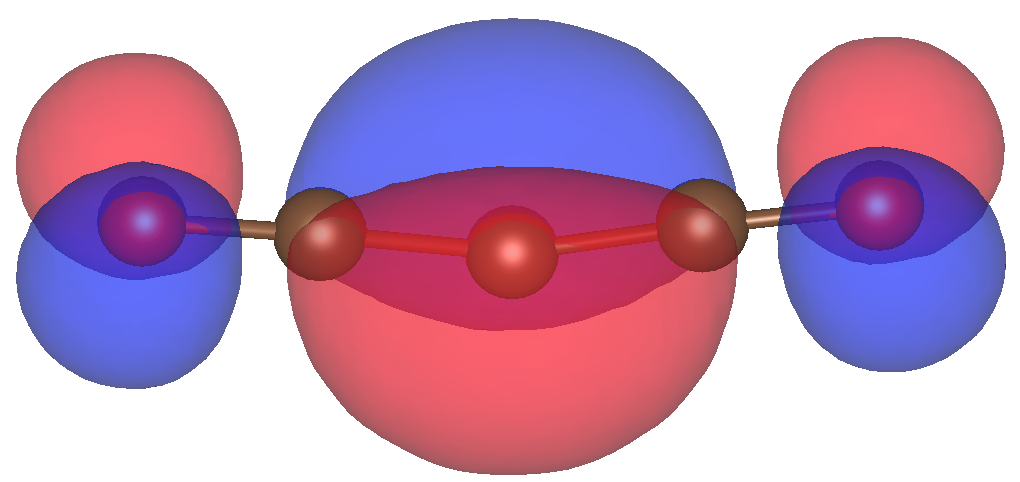
\includegraphics[width=\columnwidth]{homo3.png}
    \caption{C$_3$O$_2$ structure.}
    \label{structure}
\end{figure}
\begin{figure}
    \centering
    \includegraphics[width=\columnwidth]{bent_wings.eps}
    \caption{Results from the static calculations using the hybrid functional}
    \label{hybridresults}
\end{figure}
\begin{figure}
    \centering
    \includegraphics[width=\columnwidth]{sciresults.eps}
    \caption{Results from the static calculations using RDMFT+ACA. FIX: y-axis and font/symbol-size}
    \label{sciresults}
\end{figure}

\section{Fix:Conclusion and Outlook}

%\begin{appendix}
%\section{Changes for the single-point calculations}
%Fig. \ref{sciresults} shows the results from the static calculations using only the first bath level and 4096 Slater Determinants (out of $2^16=65536$). %The minimum appears to be around 170° as is the case for the PBE0r hybrid functional implemented by Peter.
%\subsection{Ideas for calculations to improve accuracy}
%\begin{itemize}
%    \item Increase the search space by using more Slater Determinants
%    \item Remove the friction allowing for an increase of the energy in the cntl file (as this seems to lead to high fluctuations throughout the %calculation)
%    \item Increase the bath level and see if the first bath level achieved a sufficiently good result
%    \item Do FCI on one of the geometries and compare to results from the first/second bath level energies.
%\end{itemize}
%\section{CONFIG parameters}
%
%CONFIG.H5 settings of some of the calculations were:
%\begin{itemize}
%    \item OUTER/FUNCTIONALSOLVER to 80 (to enable ACA?)
%    \item NCHIA to 8 (number of interacting orbitals)
%    \item OUTER/NCHI2 to 16 (twice the number of interacting orbitals)
%    \item INNER/TNATURAL to 1 (perform the constrained minimization in the basis of natural orbitals))
%    \item INNER/T\_FCI to 0 (0 = selected-CI, 1 = FCI)
%    \item INNER/MAXDETS to 4096 (number of Slater Determinants?)
%    \item INNER/ADDMAXDETS to 1024 (additional Slater Determinants?)
%    \item OUTER/AUGLAG/LBFGS\_TOL\_MIN to 0.0001 (some convergence criteria for the minimization)
%    \item OUTER/AUGLAG/AUGLAG\_TOL to 0.0001 (another criteria  LBFGS\_TOL\_MIN and AUGLAG\_TOL both affect the convergence of the Augmented Lagrangian?)
%\end{itemize}
%\end{appendix}
\newpage
\nocite{*}
\bibliography{references}
\end{document}
